
\documentclass[apj]{emulateapj}

\usepackage{graphicx}
\usepackage{amssymb}
\usepackage{amsmath}
\usepackage{natbib}
\usepackage{color}
\bibliographystyle{apj}
\usepackage[breaklinks,colorlinks,citecolor=blue,linkcolor=magenta]{hyperref}
\shortauthors{Zhou et al.}

%%% new command %%%
\newcommand{\ima}{\texttt{ima} files }
\newcommand{\flt}{\texttt{flt} files }
\newcommand{\eps}{$\mathrm{e}^{-}/\mathrm{s}$}
\newcommand{\tinytim}{\textit{Tiny Tim}}
\newcommand{\bpic}{$\beta$ Pic}
\newcommand{\vsini}{$v\sin i$}
\newcommand{\mjup}{M$_{\mbox{Jup}}$}
\begin{document}

\title{Discovery of Rotational Modulations in the Planetary-mass
  Companion 2M1207b: A Slow Rotation Period and Heterogeneous Clouds in a Low
  Gravity Atmosphere}
\shorttitle{Variability of 2M1207 b}
\author{Yifan Zhou\altaffilmark{1}, D\'aniel Apai\altaffilmark{1,2,3},
  Glenn Schneider\altaffilmark{1},  Mark S. Marley\altaffilmark{4}}

\altaffiltext{1}{Department of Astronomy/Steward Observatory, The
  University of Arizona, 933 N. Cherry Ave., Tucson, AZ, 85721, USA,
  \href{mailto:yifzhou@email.arizona.edu}{yifzhou@email.arizona.edu}
}
\altaffiltext{2}{Lunar and Planetary Laboratory, The University of
  Arizona, 1640 E. University Blvd., Tucson, AZ 85718, USA}
\altaffiltext{3}{Earths in Other Solar Systems Team, NASA Nexus for
  Exoplanet System Science}
\altaffiltext{4}{NASA Ames Research Center, Naval Air Station,
  Moffett Field,Mountain View, CA 94035, USA}

\begin{abstract}
  Rotational modulations of brown dwarfs have recently provided
  powerful constraints on the properties of ultra-cool atmospheres,
  including longitudinal and vertical cloud structures and cloud
  evolution. Furthermore, periodic light curve directly probes the rotational periods of ultra-cool objects.

  We present here, for the first time, time-resolved high-precision
  photometric measurements of a planetary-mass companion, 2MASS1207b,
  to a brown dwarf primary.  We observed the binary system with
  HST/WFC3 in two bands and with two spacecraft roll angles. Using
  point spread function-based photometry we reach a nearly
  photon-noise limited photometric accuracy for both components. While
  the primary is consistent with a flat lightcurve, the secondary
  shows modulations that are clearly detected in the combined
  lightcurve as well as in different subsets of the data.  The
  amplitudes are 1.45\% in the F125W and 0.92\% in the F160W filters;
  we find a consistent period of $10.2^{+0.9}_{-0.8}$ h and similar
  phase in both bands. The J- and H-band amplitude ratio of 2M1207 bis very
  similar to a field brown dwarf that has identical spectral type but
  different J-H color.  Importantly, our study also measures, for
  the first time, the rotational period for directly an imaged
  planetary-mass companion.
\end{abstract}

\keywords{brown dwarfs -- planets and satellites: atmospheres -- planets
  and satellites: individual (2M1207 b) -- techniques: photometric}
\maketitle
%
\section{Introduction}

\begin{figure*}
  \centering
  \plottwo{original}{subtracted}
  \caption{Point spread function subtraction allows isolating the
    secondary and accurately measuring its brightness in our WFC3
    F160W images. {\em Upper}: original image, the position of 2M1207
    b is indicated by a white circle.  {\em Lower:} residual image --
    after the subtraction of the hybrid PSF, 2M1207 b is detected at a
    high significant level.}
  \label{fig:1}
\end{figure*}

Presence of condensate clouds is one the most unique features of the
ultra-cool atmosphere of directly imaged exoplanet and brown
dwarfs. Studies of formation and properties of condensate clouds
\citep[e.g.][]{Ackerman2001, Burrows2006a, Helling2008, Allard2012}
have achieved great improvement in understanding the cloud behavior
across different spectral types, especially in the explanation of L-T
transition \citep[e.g.][]{Burrows2006a, Marley2010}.  Surface gravity
is suggested to be the second key parameters in defining cloud
structures \citep[e.g.][]{Marley2012} after effective temperature. Low
surface gravity objects (e.g. HR8799 bcd, \cite{Marois2008a}, 2M1207
b, \cite{Chauvin2004}) are significantly redder and under-luminous
compared to brown dwarfs.  The anomalous color and luminosity of low surface gravity
objects supports model including unusually thick clouds
\citep{Currie2011, Madhusudhan2011,Skemer2011, Skemer2012}. However, due to lack of observational
constraint, the dependence of cloud properties on surface gravity is
not very well modeled.

Intensity modulations introduced by heterogeneous clouds can be
directly observed and studied via time resolved observation and
rotational mapping. These techniques isolate the effect of cloud
properties and obtained great success in determining the rotation
period and unveiling the structures of the atmosphere of brown dwarfs
\citep[e.g.][]{Apai2013,Buenzli2012,Buenzli2015,Burgasser2013,Radigan2012,Yang2014,Metchev2015,Heinze2015}. \cite{Kostov2013}
demonstrated that these techniques can be applied to directly imaged
exoplanets, too, allowing comparative studies of objects with
different surface gravities. However, high contrast magnifies the
challenges for directly imaged exoplanets and planetary-mass
companions to acquire high-precision light curves comparing to brown
dwarfs.


  2M1207 b \cite{Chauvin2004} is the first directly imaged
planetary-mass companion. \cite{Chauvin2005,Song2006} confirmed that 2M1207 b and
its host 2M1207 A form a bound, co-moving system. 2M1207 A and
b have an angular separation of $0.78''$, which is corresponding to a
projected separation of 41.2 AU at a distance of 52.4 pc
\citep[e.g.][]{Ducourant2008}. Combining 2M1207 b's age and near infrared
luminosity with  brown dwarf cooling models
\citep[e.g.][]{Baraffe2003}, the object's mass is estimated to be
2.3-4.8 M$_{\mathrm{Jup}}$ \citep{Barman2011b}. Even though a
circumsubstellar disk was discovered around 2M1207A
\citep[][]{Sterzik2004}, the high companion-to-host
mass ratio and large separation argue for binary-like gravitational fragmentation
formation\citep{Mohanty2007}.

Early observations revealed that 2M1207 b's color is much redder and
its near-infrared luminosity is much lower than those of field brown
dwarfs with similar spectra\citep[e.g][]{Mohanty2007, Skemer2011,
  Barman2011b}. 2M1207b's luminosity -- as derived from near-infrared
photometry -- is $\sim2.5$ mag lower than that predicted based on its
mid- to late L spectral type and effective temperature of $\sim 1600$
\citep{Patience2010}.  Based multi-band near-infrared photometry
\citet{Skemer2011} argued that the apparent under-luminosity of 2M1207
b may be explained by a model of a spatially heterogeneous atmosphere
composed of patches of thin and patches of unusually thick clouds.
Similarly, \cite{Barman2011b} argued that non-local chemical
equilibrium could play an equally important role as thick clouds in
defining 2M1207b's color and luminosity.

The discovery of additional planetary-mass companions with similarly
red colors and apparent under-luminosity have highlighted 2M1207b as a
template of low gravity ultra-cool atmospheres but as of now
understanding the composition and structure of clouds and their
gravity-dependence remained elusive.



In this {\em Letter} we present the first, high-cadence,
high-precision, time-resolved {\em Hubble Space Telescope} (HST)
photometric time series of 2M1207 b, a directly imaged planetary-mass
object. We successfully detect rotational modulation and measure the
amplitudes in two bands and determine the rotational period. These observations probe the spatial heterogeneity and
vertical structure of clouds in planetary mass objects for the first
time. 

\section{Observation}



We obtained direct images of the 2M1207A+b system on UT 2014 April 11
from 08:07:47 to 16:53:18 using HST and its Wide Field Camera 3
\citep[WFC3, pixel scale=$0.130$mas/pixel, ][]{Mackenty2008} in the frame of
the HST Program GO-13418 (PI: D. Apai). We acquired the observations
in filters F125W ($\lambda_{\mathrm{pivot}}$ = 1245.9 nm, full width
at half maximum (FWHM) = 301.5 nm) and F160W
($\lambda_{\mathrm{pivot}}$ 1540.52, FWHM = 287.9 nm), roughly
corresponding to the J and H bands. We used the $256\times256$ pixels
sub-array mode to avoid memory dumps during the observations.  In
order to provide a near-continuous coverage for detecting modulations
we observed the 2M1207 system in 6 consecutive HST orbits, obtaining
data with cadence of $\sim1.5$ minutes over a baseline of 8 hours and
40 minutes. The observations were interrupted by 58 minutes long Earth
occultations every 94 minutes.

The observations applied space craft rolls each two orbit to allow
roll-subtraction of the primary \citep[e.g.][]{Song2006}. The
telescope roll angles for orbit 1, 3, and 5, and those for 2, 4, and 6
differ by $25^{\circ}$. At the separation of 2M1207 b, this angle
difference corresponds to a displacement of $0.34''$, or 2.75 and 2.30
resolution elements in F125W and F160W, respectively. In each orbit we
took 8 SPARS10 exposure sequence with NSAMP=10, alternating between
F160W and F125W filters, with 2--3 identical exposures in each
exposure sequence. To improve sampling and reduce the risk that the
core of point spread function (PSF) is affected by bad pixels, we
applied a 4-point dither pattern with differential "X/Y" offsets of
1.375" in the detector frame, providing optimal non-integral (half
pixel) step of 10.5 and 8.5 pixels in F125W and F160W,
respectively. In total, we obtained 70 images with 10 non-destructive
read-outs in F125W and 64 images in F160W with exposure time of 88.4~s
for both filters.

\section{Data Reduction}



\subsection{Photometry}

We started the reduction from the \flt{} produced by the WFC3's
\texttt{calwfc3} pipeline. We did not opt to use \ima{} that contain
all non-destructive read-outs, because they provided less information
on 2M1207A, which saturated after the first few samples.  The \flt{}
are results of basic calibration, including dark current correction,
non-linearity correction, flat field correction, as well as
up-the-ramp fit on the non-destructive read-outs. 
Pixels with data quality flags ``bad detector pixels'', ``unstable
response'', and ``bad or uncertain flat value'' were masked out and
excluded from further analysis as suggested by previous transit
exoplanet spectroscopic observations\citep[e.g.][]{Berta2012,
  Kreidberg2014}.


The major challenge of high contrast observation with WFC3/IR is the
fact that the detector is significantly under-sampled.  2M1207 A and b
are only separated by $\sim6$ pixels or $\sim$5 FWHM of the PSF on the
detector. When
applying roll subtraction, notable artifacts are introduced by image
shifting and interpolation.  \tinytim{} PSF
simulator\citep{Krist1995} offers a solution by providing Nyquist or
better sampled PSF, but systematic errors of \tinytim{} PSF for WFC3
limits its ability in high precision photometry\citep{Biretta2014}.
Building on the large number of PSFs obtained in our program at two
different roll angles, we followed a novel, two-step approach that
uses a hybrid PSF, {\color{blue}which combined the strengths of the roll
subtraction-based and the simulated PSF-based approaches.}
First, based on our observations we observationally derived correction maps
for \tinytim{} that accurately described the scattered light component
for the primary at the correct location on the detector. Second, we
carried out a PSF-photometry using hybrid PSFs composed by \tinytim{}
PSFs and the correction map  by simultaneously
minimizing the residuals from the primary and the secondary.
% However, we are able to fully characterize the difference of model
% and observed PSFs with 6 orbits time-resolved observation data. To
% obtain robust \tinytim{} PSF photometry, we design a 2-round PSF
% fitting strategy: 1. calculating correction map for \tinytim{};
% 2. hybrid PSF photometry.

For both of 2 steps, we used \tinytim{} to calculate 10$\times$
over-sampled model PSFs based on the filters, the spectra (2M1207A:
\cite{Bonnefoy2014}, 2M1207 b: \cite{Patience2010}), the telescope's
actual focus, and the telescope jitter.  We used the set of \tinytim{}
parameters provided by \cite{Biretta2014} to improve modeling the cold
mask, diffraction spikes, and the coma. The focus parameters are are
interpolated to the precise time of the observations using the
tabulated values provided by
STScI\footnote{\url{http://www.stsci.edu/hst/observatory/focus/FocusModel}}.
To align the \tinytim{} PSF to the observed PSF of 2M1207 A, we
moved the over-sampled PSF on a coordinate grid (gird size=0.001 pixel)
using cubic interpolation, and searched for the position that minimizes
the rms difference of the observed and the re-binned \tinytim{} PSF over
a region centered on 2M1207 A with a 5-pixel-radius aperture centered
on 2M1207 b excluded.  Then we introduced another \tinytim{} PSF for
2M1207 b and fit the position of 2M1207 b and the scales of the
\tinytim{} PSFs of 2M1207 A and b simultaneously by minimizing the
residual from both primary and secondary. In the first step, we discovered that the
difference of observed PSFs and model PSFs were very stable for a
specified telescope roll angle and dithering position. Therefore, at the end of the first step,
we derive 8 (2 roll angles $\times$ 4 dithering positions) correction
maps for each filter:
\begin{equation}
  \mathrm{Corr = Median(PSF_{obs.} - PSF_{model} )}
\end{equation}
where $\mathrm{PSF_{model}}$ was a combination of two scaled \tinytim{} PSFs
for 2M1207 A and b. In the second round, we combined the correction
map linearly with the two \tinytim{} PSFs to generate hybrid PSFs,
and scaled the correction map together with the two PSFs so that the
residual which is expressed as
\begin{equation}
  \mathrm{residual} = \mathrm{Image} - a\cdot \mathrm{PSF_{A}} - b\cdot
    \mathrm{PSF_{b}}- c\cdot\mathrm{ Corr}
  \end{equation}
  is minimized by least square fitting.
We found that by introducing the correction term,
the reduced $\chi^{2}$ was decreased from $\sim 10$ to
$\sim 1$. Relative photometry was acquired from the scaling
parameters of the \tinytim{} PSFs.


Our final step was to correct for a slight apparent trend between the
position of the targets on the detector and their flux. We attributed
this to a combination of slight changes in the PSF profile due to
pixelation and to the effect of imperfectly corrected pixel-to-pixel
sensitivity variations. We corrected for these apparent
position-dependent flux changes by normalizing each photometric point
by the median of all fluxes measured when the target was at the
same position, i.e. combining data over 6 orbits.  We note that this
correction is small and, as we demonstrate in the next sections,
cannot introduce artificial modulations that resemble the long-period
variations we identify in 2M1207b. 

% PSF profiles change with exposure positions due to
% pixelation, especially for the case that WFC3 IR is significantly
% under-sampled. Also, the flat fields may potentially have large scale
% structures \citep{dressel2012wide}. We find a correlation of
% photometry with PSF positions on detector frame for both 2M1207 A and
% b. Correction is made by normalizing each group of
% exposures that have the same dithering position and telescope roll angle
% individually -- we take the median of the fluxes that are measured
% from these exposures as normalization factors and divided them from
% every photometric measurement. Because the normalization factor for
% each group of exposures is calculated across the whole observation in
% time domain,
% this step has negligible impacts on variability
% analysis.



As our study is the first to present high-contrast, high-cadence
observations, we provide a detailed analysis of the uncertainties and
their impact on our results.

\subsection{Uncertainty Analysis: White noise}

First we estimated the photon noise for the photometry of
2M1207 b. The total photon noise of the photometry was calculated by
combining the photon noise of every pixel, which was derived
from count rates and detector gain. The photon noises 
in F125W and F160W are 1.33\% and 1.02\%, respectively.

Since the PSFs for the 2M1207 A and b were fitted simultaneously, the
uncertainties for photometry and position of the primary and secondary
were coupled. Errors in position measurements of 2M1207 A could
potentially affect the photometry of 2M1207 b. We used a Monte Carlo
(MC) method to evaluate the overall systematic of the PSF fitting. We
applied photometry to images that were added with random
Poisson noise and repeated the photometry procedure for 1000 times. The
uncertainties for F125W and F160W photometry were found to be 1.34\% and 1.12\%,
respectively. 

\subsection{Uncertainty Analysis: Flat field uncertainties}


A further contribution to photometric uncertainties may be introduced
by imperfectly corrected pixel-to-pixel sensitivity
differences. 2M1207 b were observed at 8 different positions on the
detector (2 rolls $\times$ 4 dithering positions). Imperfect flat
field correction could introduce position-dependent
differences in the count rates. The uncertainty of WFC3 IR flat field
is typically $\sim 1\%$ \citep{dressel2012wide}.

In PSF photometry, however, multiple pixels are fitted simultaneously,
so that we expect the photometry to be less affected by high spatial frequency flat field
noise, and have a lower than 1\% uncertainty from the flat field
errors. To verify this, we multiplied every image by an artificial flat
field error mask (AFEM) -- a uniformly distributed Gaussian noise array with
mean of 1 and sigma of 1\% -- and repeated the PSF photometry on the
resulting images.  The analysis of these experiments resulted in almost
identical light curve to the original, verifying that the flat field
errors did not affect our photometry significantly (Figure
\ref{fig:2}, bottom panel).


\section{Verification of Photometric Modulations and Amplitude
  Estimate}

 \begin{figure*}
  \centering
  \plotone{systematics}
  \caption{F125W (left) and F160W (right) light curves under different
    variability verification tests. Individual measurements are
    plotted with gray crosses. Photometric measurements of the same exposure
    sequence are binned, and binned photometry are plotted with points
    or squares. Best fitted sinusoidal curves are plotted with solid
    lines. {\em Upper}: binned measurements taken in dithering
    position 1 and 3 (red points) and that taken in 2 and 4 (blue
    squares) are plotted with different symbols. They demonstrate same
    trend of modulation. In upper left panel, green line is sinusoidal
    wave fitted with all parameter set free, and purple line is
    sinusoidal wave fitted with period set the same as that of
    F125W. {\em Middle}: sinusoidal waves fitted without using the
    data taken in Orbit \#1. These curves are almost identical to the
    curves plotted in upper panel. {\em Lower}: photometry measured
    with AFEM-added images and best fitted sinul curves. These
    points and curves are also almost identical to those plotted
    in the upper panel.}
  \label{fig:2}
\end{figure*}

\subsection{Tests and Verification}

The light curves that resulted from our photometry showed apparently
sinusoidal modulations, discussed in more details in
\S,\ref{Results}. To verify that these modulations are intrinsic to
the object and not results of our data reduction procedures or due to
instrumental changes, we carried out three different tests.

First, we fitted sinusoids independently to the light curves of two
filters to verify the similarity of the signal in the two bands
(Figure \ref{fig:2}, top panel). Inconsistent periods or light curve
shapes would argue against a genuine signal.  We found that the periods
of the best fit sine waves were similar, $10.5^{+1.2}_{-1.3}$h for
F125W and $9.1^{+1.1}_{-1.0}$h for F160W. These periods are consistent
within the uncertainty. Furthermore, these periods are not close to
any timescales over which HST or WFC3 changes, and are
very different from all timescales present in our observations
(dithering timescales, integration times, and orbital timescales).

As a second test, we repeated the analysis neglecting the first
orbit. The motivation behind this test is that, due to spacecraft
thermal settling, the first orbits of HST observations are often
slightly unstable, and neglected in high-precision studies
\citep[e.g.][]{Mandell2013}. Indeed, in our analysis 2M1207 A is
significantly fainter in the first orbit (Figure \ref{fig:3}) than in
the subsequent ones.  Our analysis based on orbits 2--6 found
essentially identical results to our analysis using the whole 6 orbits, based on
which we conclude that the first less reliable orbit does not affect
our results significantly (Figure \ref{fig:2}, middle panel).

As a third test, we explored whether a subset of images, perhaps due to
imperfectly normalized or correlated with specific instrument states,
could drive the light curves into an apparently sinusoidal shape. To
test this possibility, we split the data into two temporally
overlapping halves: subset one were images taken at dithering position
1 and 3, and subset two were those taken at dithering position 2 and
4. For both subsets, we repeated our analysis independently.  For both
of F125W and F160W, two halves demonstrated similar sinusoidal
modulations.  Our analysis detect sinusoidal modulations in {\em both}
subsets and in {\em both} filters, with periods and amplitudes
consistent with those derived from the complete data set (Figure
\ref{fig:2}, upper panel).
 
 These tests demonstrate that the modulation seen in our data are
 consistently present in the different filters, in the different time
 segments of the data, and in data obtained in different dithering
 positions. All of the three tests support the signal to be
 intrinsic to the target. 
 

\subsection{Amplitude and Period Measurements}

We used a MC method to analyze the light curve, and provided amplitudes
and periods as well as their uncertainties for both filters. We
generated series of Gaussian distributed random noise with standard deviation
same as the photon noise, add the noise to the original light curves, and
fit sinusoids to the newly combined light curves. We repeated these
procedures  for 100,000 times and obtain the distributions of period
and amplitude (Figure \ref{fig:4}).


\section{Result}
\label{Results}

  \begin{figure*}
  \centering
  \plotone{sineCurveFit_binCombined}
  \caption{Normalized light curves for 2M1207 B (upper) and A (lower)
    with filter F125W (left) and F160W (right). Individual photometric
  measurement are plotted in gray crosses and binned photometry are
  plotted with red points. Best fitted sinusoidal waves are plotted
  with blue solid lines.}
  \label{fig:3}
\end{figure*}

\begin{figure*}
  \centering
  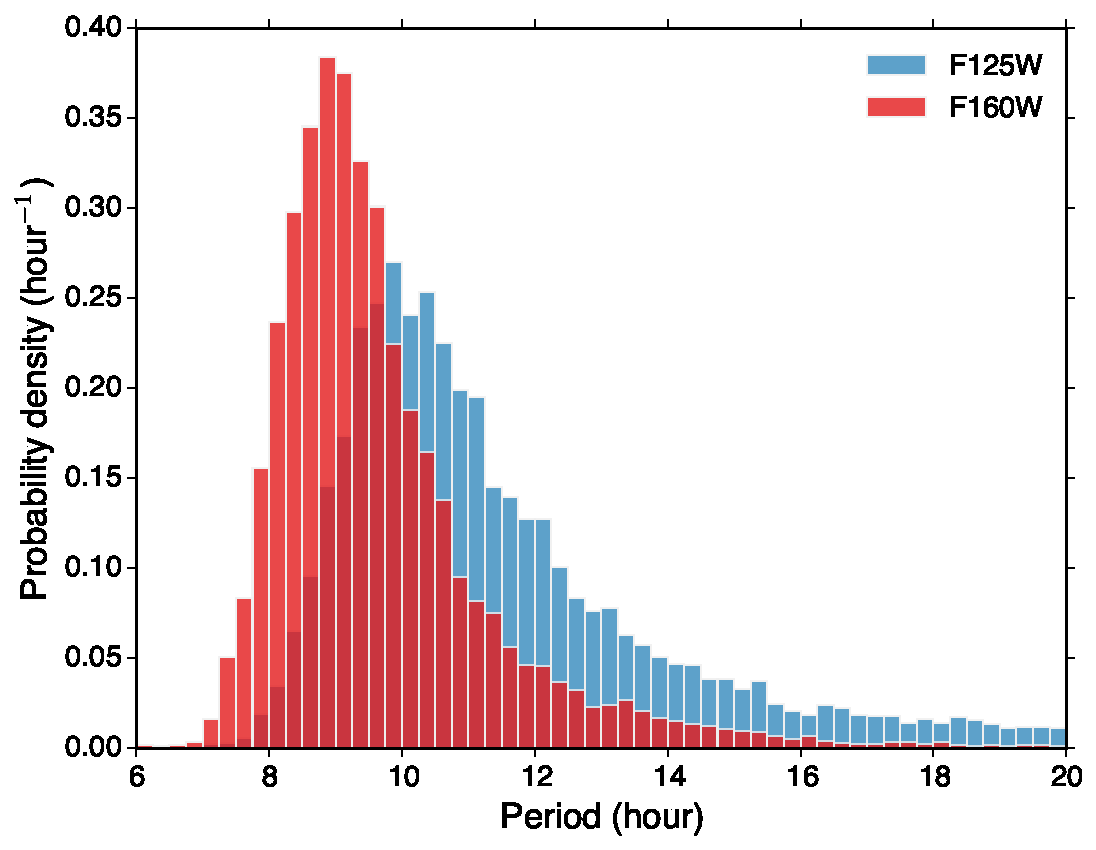
\includegraphics[width=0.45\textwidth]{periodDistr}
  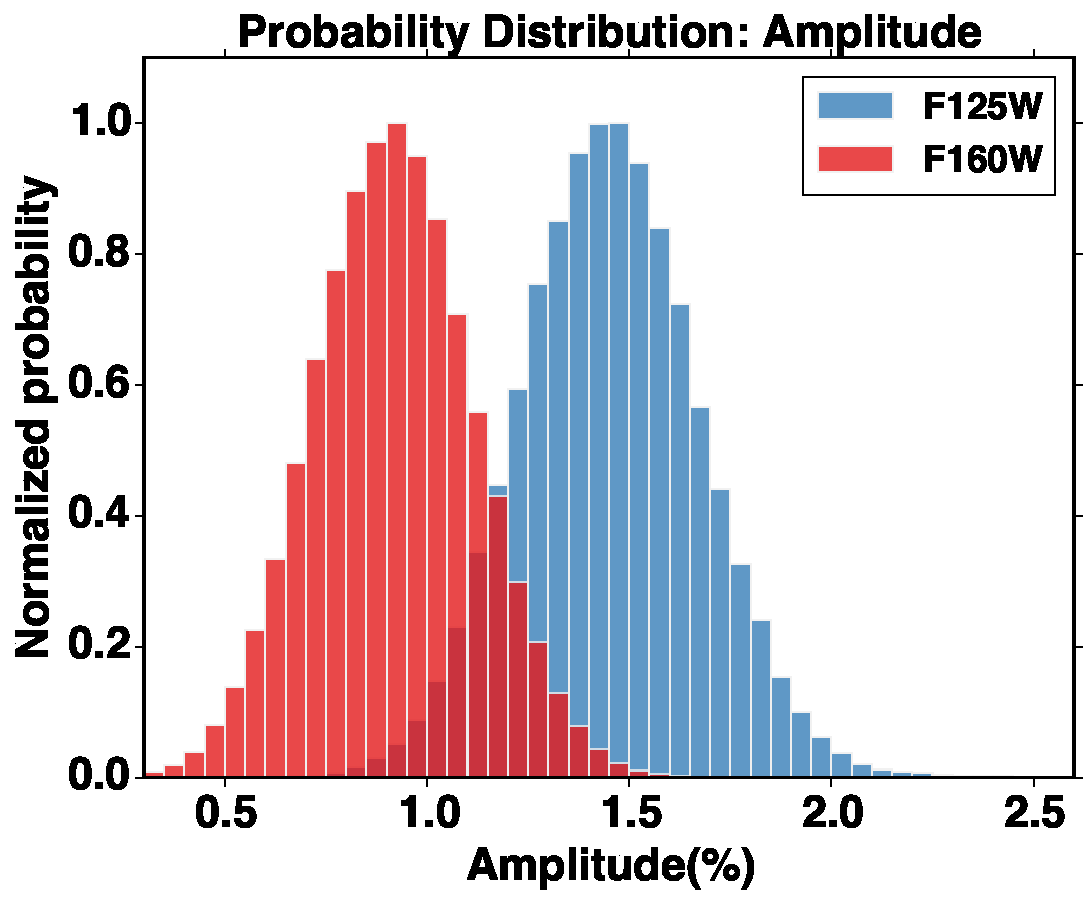
\includegraphics[width=0.45\textwidth]{amplitudeDistr}
  \caption{Distributions for periods (left) and amplitudes(right) for the light
    curve of F125W and F160W. The bin size for histograms of period is
  0.25 hour and for that of amplitude is 0.5\%. Histograms are
  normalized to the maximum. In the right panel, Gaussian profiles are fitted to the
  histograms of periods and plotted in solid lines.}
  \label{fig:4}
\end{figure*}

We present the first high-resolution, high-cadence, and high-precision
photometry of a directly imaged planet or planetary-mass
companion. Our observations reveal a modulation in the light curve of
the $\sim 4 \mathrm{M_{{Jup}}}$ companion 2M1207 b, the first detection
of modulations in directly imaged planetary-mass objects.  The best
fit periods for F125W and F160W are $10.5_{-1.2}^{+1.3}$ and $9.1_{-1.0}^{+1.1}$ hour,
respectively. We also fit the two band light curves together forcing the
periods of two sinusoids to be the same, and obtained a period
of $10.2^{+0.9}_{-0.8}$. The amplitudes for the normalized light
curves are 1.45\% and 0.92\% for F125W and F160W, respectively.

We obtained high signal to noise photometry for both 2M1207 A
and B (Figure \ref{fig:3}). On average, the photometric contrast is
$6.52\pm0.01$ mag for F125W and $5.77\pm0.01$ mag for F160W.


%  With 64\% confidence,
% we estimate the 1-$\sigma$ range for the periods of F125W and F160W
% to be  and  h,
% respectively. The period of best fitted sinusoid for F125W light curve
% is 1.5h longer than that for F160W, which is $\sim 20\%$ larger than
% 1-$\sigma$. We also jointly fit the two band light curves forcing the
% periods of two sinusoids to be the same. We derive a modulation period of $10.2^{+0.9}_{-0.8}$ h.

We  found that the amplitudes in the two bands are
significantly different. By fitting Gaussians to the MC fit result
distributions, we determined that the  amplitude for F125W is
1.45\% with a standard deviation of 0.22\%, and  the amplitude for F160W is
0.92\% with a standard deviation of 0.20\%. The amplitudes of two
bands are separated by more than 2-$\sigma$ The amplitude
for F125W is 1.58 times of that for F160W light curve.


\section{Discussion}

\begin{figure*}
  \centering
  \plottwo{rotationDiagram}{JH}
  \caption{comparison of 2M1207's rotation period and color change
    with brown dwarfs, \bpic{} b, and solar system planets. {\em
      Left}: period vs. mass plot for 2M1207 b (red square), solar
    system planets and \bpic{} b (blue squares), and brown dwarfs
    (black circles, gray shade). Final rotation rates for 2M1207 b and
    \bpic{} b estimated by conservation of angular momentum are
    plotted with faint red and blue squares, respectively. The mass of brown dwarfs are assumed
    to be 30 \mjup{}. The gray rectangle that has a $\pm$15 \mjup
    range in $x$, and a $\pm \sigma$ of brown dwarf periods range in
    $y$, indicates a region where brown dwarfs most likely to appear
    in this diagram. Rotation period monotonically decreases with the
    increase of mass. {\em Right}: ratio of modulation amplitude in J
    and H band vs. spectral type for 2M1207 b and brown dwarfs. The
    point for 2M1207 b is shifted to +$x$ for half spectral type for
    clarification.  The colors of the points represent J$-$H
    magnitude, and the sizes of the points are proportional to the
    J-band modulation amplitudes. The gray dashed line is the result
    of a linear fit to these points. Tight correlation of J- and
    H-band modulation amplitude ratio and spectral type is shown.}
 \label{fig:5}
\end{figure*}

% A fundamental result of our study is the direct determination of the
% rotation period of a directly imaged planetary-mass object. We
% convert the rotation period to equatorial velocity  by adopting a radius of 1 -- 1.4
% $R_{\mathrm{Jup}}$ for 2M1207 b, and 1 $R_{\mathrm{Jup}}$ for field
% brown dwarfs with well defined rotation period from the study of
% \cite{Metchev2015}, and compare their rotation velocities with solar
% system planets and \bpic{} b in the left
% panel of Figure \ref{fig:5}.  The study by
% \citep[][]{Snellen2014} succeeded in measuring \vsini{} for \bpic{} b
% and demonstrated that it fits a trend defined by Solar System planets
% in which more massive planets have faster rotation rates. They suggested
% that this relation is linked to the accretion processes during planet
% formation.

An important result of our study is the direct measurement of the
rotation period of a directly imaged planetary-mass object. In the
left panel of Figure~\ref{fig:5} we compare the rotation period of
2M1207 b to the solar system planets, \bpic{} b the only other directly
imaged planet with an estimated period and measured \vsini, and
field brown dwarfs from the study of
\cite[][]{Metchev2015}. \cite[][]{Snellen2014} measured \vsini{} 
for \bpic{} b and demonstrated that it fits a trend defined by Solar
System planets in which more massive planets have faster rotation
rates. The interesting finding that \bpic{} b, an exoplanet that formed
in a protoplanetary disk, follows this trend suggests a possibly
connection between planet mass, initial angular momentum, and
formation in a disk.

Excitingly, our measurement of the rotation period of 2M1207 b, a
planet mass companion that has similar age to \bpic{} b, has a
rotation period that fits in the same trend, as well as majority of
brown dwarfs. As 2M1207 b and \bpic{} b evolve and cool down, they are
expected to shrink to the size of Jupiter. Order of magnitude
estimation based on the conservation of angular momentum results in
final rotation periods of $\sim 5$ h and $\sim 3$ h
\citep{Snellen2014} for 2M1207 b and \bpic{} b, respectively, which
still fit to the period vs. mass trend. Although 2M1207 A is known to
host a circumsubstellar disk \citep{Sterzik2004}, the low mass of
typical brown dwarf disks \citep[e.g.]{Klein2003, Mohanty2013} and its
large separation argue against the possibility that 2M1207b has formed
in a protoplanetary disk.  The result that objects formed in different
scenarios share the same trend of period vs. mass suggests that
rotation periods -- in absence of well-determined ages -- may
contribute insufficient evidence for a formation in a disk vs. in a
cloud core environment. Although rotation rates may have limited value
for deciphering formation pathways, measurements of mass, age, and
rotation periods will map the angular momentum evolution of
planetary-mass objects and may place powerful constraints on the
evolution of the internal structures of these contracting objects.
%{\em Add younger BDs and this may change}
% Excitingly, our measurement of the rotation period demonstrates that
% 2M1207 b, a planetary-mass companion  with similar age to \bpic{} b, has a rotation velocity
% that fits in the same trend, as well as majority of brown
% dwarfs. We note that 2M1207 b is most likely formed in the same way as brown
% dwarfs by gravitational fragmentation, which suggests
% that rotation periods are not good tracers of the formation pathways
% and may not contribute important evidence for a formation in a disk
% vs. in a cloud core environment.

Our inferred rotation period is very similar to those of Jupiter and Saturn, which
have periods of 9.9 and 10.5 hours, respectively.   Moreover, our inferred rotation 
is sufficiently fast that--just as with Jupiter and Saturn--the atmospheric dynamics 
is likely to be rotationally dominated at regional to global scales \citep[][]{Showman2013}.  
The importance of rotation can be characterized by the Rossby number 
$Ro = U/\Omega L$, where $U$ is the characteristic wind speed, $\Omega$ is the 
angular rotation rate ($1.7\times10^{-4}\rm\,s^{-1}$ for a 10-hour rotation period), 
and $L$ is the characteristic horizontal length scale.   Although the wind speeds are 
unknown, \citet[][]{Showman2013} presented a theory of the atmospheric circulation 
on brown dwarfs and directly imaged giant planets, which predicts wind speeds in the 
range of tens to hundreds of $\rm m\,s^{-1}$ depending on parameters.   Global 
simulations of the atmospheric circulation using a one-layer model by 
\citet{Zhang2014} predict a similar range.  Considering wind speeds ranging 
from  10 to $1000\rm\,m\,s^{-1}$, a circulation that is global in scale (L=Jupiter radius) 
implies Rossby numbers of 0.001 to 0.1 on 2M1207b (see Figure 1 in \citet{Showman2013}).  For a circulation whose length scale is 0.1 Jupiter radii, the Rossby numbers 
would range from 0.01 to 1 depending on wind speed.  Thus, over almost the full 
range of plausible parameters, we expect that the large-scale circulation on 
2M1207b---like Jupiter, Saturn, and most brown dwarfs---exhibits a Rossby number 
much less than one.  This implies that the atmospheric circulation is rotationally dominated 
and that the horizontal force balance is approximately geostrophic, that is, a balance 
between Coriolis and pressure-gradient forces.    

From the perspective of atmospheric dynamics, 2M1207b exhibits other important 
similarities to brown dwarfs.  Its high effective temperature indicates that--like most 
brown dwarfs--2M1207b exhibit a strong interior heat flux presumably transported by 
convection, and that, by comparison, the external irradiation is negligible to the circulation.  
These similarities suggests that the overall dynamical mechanisms for driving an atmospheric 
circulation on 2M1207b should be similar to those on brown dwarfs.  Thus, given the
prevalence of IR light curve variability observed on brown dwarfs, it is unsurprising to
find such variability on directly imaged planets like 2M1207b.  Nevertheless, directly
imaged planets generally have lower gravity than field brown dwarfs, and this will 
affect the details of the atmospheric circulation, potentially including the cloud patchiness.  
Further observations of 2M1207b and other directly imaged planets will help to 
elucidate these differences.   Key questions for the future will include assessing the 
extent to which the atmospheric circulation on 2M1207b--including the 
existence of absence of zonal (east-west) jet streams, vortices, storms, and turbulence, 
and their effect on cloud patchiness--are similar or different than that on typical field 
brown dwarfs.

Furthermore, our observations allow us to compare the relative
amplitudes in the J- and H-bands with the handful of brown dwarfs
for which high-quality near-infrared time-resolved observations have
been obtained. In the right panel of Figure \ref{fig:5}, we compare the
relative amplitude of J- and H-bands of 2M1207 b and brown dwarfs
\citep{Apai2013,Buenzli2012,Buenzli2015,Burgasser2013,Radigan2012,Yang2014} that
have different spectral types and J$-$H colors.

We also find an interesting possible correlation between the spectral types of the
objects and their J- to H-band amplitude ratios. In the right panel of
Figure \ref{fig:5}, we show that earlier spectral type objects
have larger amplitudes at shorter wavelength than at longer
wavelengths. Interestingly, although the J$-$H color of 2M1207 b is
significantly redder, its relative amplitude ratio is very similar to
that of 2M1821, which also has an L5 spectral type \cite{Yang2014}.
This exciting, but tentative trend must be confirmed on a larger sample of source that also
sample a broader range of surface gravities as well as spectral types.
If the larger sample verifies the trend suggested by our small sample,
the amplitude ratio will provide a powerful probe of the spectral type
and surface gravity dependence of vertical cloud structure. 

% {\color{red}This trend can be qualitatively explained using the toy model proposed
% in \cite{Yang2014} within the spectral type range of mid-L to L-T
% transition. Assuming that intensity modulations are introduced by a
% refractory cloud whose upper layer locates at altitude $z$, the
% amplitude ratio for J and H band can be expressed as
% $\mathrm{Amp_{J}}/\mathrm{Amp_{H}} =
% \exp\left[-(\tau_{\mathrm{J}}(z)/\tau_{{\mathrm{H}}}(z)\right]$,
% where $\tau_{\mathrm{J}}(z)$ and $\tau_{\mathrm{H}}(z)$ are the
% optical depths of upper cloud layer for J and H bands. The opacity for
% J band is smaller than that for H, therefore from mid-L to L-T
% transition, as the cloud upper boundary appears higher in the
% atmosphere, the optical depth difference for the two bands gets
% smaller, and the amplitude ratio decreases.  We note, that the late T
% dwarf 2M2228 falls exactly on this trend, but whose variations are
% likely to emerge from a different mechanism as their silicate clouds
% are below the visible photosphere \citep[e.g.][]{Stephens2009}.

% We infer that the upper cloud layer of 2M1207 b is at a similar optical
% depth as that of a matching spectral type field brown dwarf from the fact
% that they share similar J- and H-bands light curve amplitude ratio.
% The
% two processes that atmosphere opacity at certain pressure level
% enhances and the cloud thickness increases with the decrease of surface
% gravity have to counterbalance with each other to maintain the optical
% depth of the cloud upper layer.}



\section{Conclusions}
In summary, from our J- and H-band high precision, high-cadence light
curves we discovered sinusoidal modulations in the planetary-mass
object 2M1207 b. This is the first detection of rotational modulations
in a directly imaged planetary-mass object.  The period is
$10.2^{+0.9}_{-0.8}$, similar to that derived from \vsini{} 
measurements for the directly imaged exoplanet \bpic{} b and
significantly longer than most field brown dwarfs with known rotation
periods. The amplitude ratio of J and H band is very
similar to that of a field brown dwarf with identical L5 spectral type, although they have
very different J$-$H colors.

Finally, we note that the observations presented here open an exciting
new window on directly imaged exoplanets and planetary-mass
companions. Our study demonstrates a successful application of
high-cadence, high-precision, high-contrast photometry with planetary
mass companion. We also show that these observations can be carried
out simultaneously at multiple wavelengths, allowing us to prove
multiple pressure levels. With observation of a larger sample and at
multiple wavelengths, we will be able to explore the detailed
structures of atmospheres of directly imaged exoplanets, and identify
the key parameters that determine these.

Support for program number 13418 was provided by NASA through a grant
from the Space Telescope Science Institute, which is operated by the
Association of Universities for Research in Astronomy, Inc., under
NASA contract NAS5-26555. The results reported herein benefitted from
collaborations and/or information exchange within NASA's Nexus for
Exoplanet System Science (NExSS) research coordination network
sponsored by NASA's Science Mission Directorate. M.S.M. acknowledges
support from the NASA Astrophysics Theory Program.
\bibliography{ref.bib}
\end{document}

%%% Local Variables:
%%% mode: latex
%%% TeX-master: t
%%% End:
